\documentclass[12pt]{report}
\usepackage[utf8]{inputenc}
\usepackage[russian]{babel}
%\usepackage[14pt]{extsizes}
\usepackage{listings}
\usepackage{graphicx}
\usepackage{amsmath,amsfonts,amssymb,amsthm,mathtools} 
\usepackage{pgfplots}
\usepackage{filecontents}
\usepackage{indentfirst}
\usepackage{eucal}
\usepackage{float} 
\usepackage{amsmath}
\usepackage{enumitem}
\usepackage[justification=centering]{caption} 
\usepackage{tikz}
\usepackage{pgfplots}
\pgfplotsset{compat=newest}

\frenchspacing

\usepackage{indentfirst} % Красная строка


%\usetikzlibrary{datavisualization}
%\usetikzlibrary{datavisualization.formats.functions}

\usepackage{amsmath}


% Для листинга кода:
\lstset{ %
language=haskell,                 % выбор языка для подсветки (здесь это С)
basicstyle=\small\sffamily, % размер и начертание шрифта для подсветки кода
numbers=left,               % где поставить нумерацию строк (слева\справа)
numberstyle=\tiny,           % размер шрифта для номеров строк
stepnumber=1,                   % размер шага между двумя номерами строк
numbersep=5pt,                % как далеко отстоят номера строк от подсвечиваемого кода
showspaces=false,            % показывать или нет пробелы специальными отступами
showstringspaces=false,      % показывать или нет пробелы в строках
showtabs=false,             % показывать или нет табуляцию в строках
frame=single,              % рисовать рамку вокруг кода
tabsize=2,                 % размер табуляции по умолчанию равен 2 пробелам
captionpos=t,              % позиция заголовка вверху [t] или внизу [b] 
breaklines=true,           % автоматически переносить строки (да\нет)
breakatwhitespace=false, % переносить строки только если есть пробел
escapeinside={\#*}{*)}   % если нужно добавить комментарии в коде
}

\usepackage[left=2cm,right=2cm, top=2cm,bottom=2cm,bindingoffset=0cm]{geometry}
% Для измененных титулов глав:
\usepackage{titlesec, blindtext, color} % подключаем нужные пакеты
\definecolor{gray75}{gray}{0.75} % определяем цвет
\newcommand{\hsp}{\hspace{20pt}} % длина линии в 20pt
% titleformat определяет стиль
\titleformat{\chapter}[hang]{\Huge\bfseries}{\thechapter\hsp\textcolor{gray75}{|}\hsp}{0pt}{\Huge\bfseries}


% plot
\usepackage{pgfplots}
\usepackage{filecontents}
\usetikzlibrary{datavisualization}
\usetikzlibrary{datavisualization.formats.functions}

\begin{document}
%\def\chaptername{} % убирает "Глава"
\thispagestyle{empty}
\begin{titlepage}
	\noindent \begin{minipage}{0.15\textwidth}
	
\includegraphics[width=\linewidth]{b_logo}
	\end{minipage}
	\noindent\begin{minipage}{0.9\textwidth}\centering
		\textbf{Министерство науки и высшего образования Российской Федерации}\\
		\textbf{Федеральное государственное бюджетное образовательное учреждение высшего образования}\\
		\textbf{~~~«Московский государственный технический университет имени Н.Э.~Баумана}\\
		\textbf{(национальный исследовательский университет)»}\\
		\textbf{(МГТУ им. Н.Э.~Баумана)}
	\end{minipage}
	
	\noindent\rule{18cm}{3pt}
	\newline\newline
	\noindent ФАКУЛЬТЕТ $\underline{\text{«Информатика и системы управления»}}$ \newline\newline
	\noindent КАФЕДРА $\underline{\text{«Программное обеспечение ЭВМ и информационные технологии»}}$\newline\newline\newline\newline\newline
	
	
	\begin{center}
		\noindent\begin{minipage}{1.3\textwidth}\centering
			\Large\textbf{  Отчёт по лабораторной работе №6}\newline
			\textbf{по дисциплине "Анализ алгоритмов"}\newline\newline
		\end{minipage}
	\end{center}
	
	\noindent\textbf{Тема} $\underline{\text{Муравьиный алгоритм и метод полного перебора для решения задачи коммивояжёра}}$\newline\newline
	\noindent\textbf{Студент} $\underline{\text{Варламова Е. А.}}$\newline\newline
	\noindent\textbf{Группа} $\underline{\text{ИУ7-51Б}}$\newline\newline
	\noindent\textbf{Преподаватели} $\underline{\text{Волкова Л.Л.}}$\newline\newline\newline
	
	\begin{center}
		\vfill
		Москва~---~\the\year
		~г.
	\end{center}
\end{titlepage}

\setcounter{page}{2}
\tableofcontents
\newpage
\chapter*{Введение}
\addcontentsline{toc}{chapter}{Введение}
	
Муравьиный алгоритм -- один из эффективных полиномиальных алгоритмов для нахождения приближённых решений задачи коммивояжёра, а также решения аналогичных задач поиска маршрутов на графах. Суть подхода заключается в анализе и использовании модели поведения муравьёв, ищущих пути от колонии к источнику питания, и представляет собой метаэвристическую оптимизацию.
	
\section*{Цель лабораторной работы}
	
Целью данной лабораторной работы является изучение муравьиного алгоритма и приобретение навыков параметризации методов на примере муравьиного алгоритма.
	
\section*{Задачи лабораторной работы}
	
В рамках выполнения работы необходимо решить следующие задачи:
	
\begin{itemize}
	\item решить задачу коммивояжера при помощи алгоритма полного перебора и муравьиного алгоритма;
	\item реализовать алгоритмы полного перебора и муравьиный алгоритм для решения задачи коммивояжёра;
	\item замерить и сравнить время выполнения реализаций алгоритмов;
	\item провести параметризацию реализации муравьиного алгоритма;
	\item сделать выводы на основе проделанной работы.
\end{itemize}

\chapter{Аналитическая часть}
	
В данном разделе представлены теоретические сведения о рассматриваемых алгоритмах.

Задача коммивояжёра -- поиск минимального гамильтонова пути во взвешенном графе.

\section{Полный перебор}

Пронумеруем все города от 1 до $n$. Базовому городу присвоим номер n. Каждый тур по городам однозначно соответствует перестановке целых чисел $1, 2, ..., n$.

Задачу коммивояжера можно решить образуя все перестановки первых $n$ целых положительных чисел. Для каждой перестановки строится соответствующий тур и вычисляется его стоимость. Обрабатывая таким образом все перестановки, запоминается тур, который к текущему моменту имеет наименьшую стоимость. Если находится тур с более низкой стоимостью, то дальнейшие сравнения производятся с ним.

Сложность алгоритма полного перебора составляет $O(n!)$, где $n$ -- число городов.
	
\section{Муравьиный алгоритм}

Моделирование поведения муравьев связано с распределением феромона на тропе — ребре графа в задаче коммивояжера. При этом вероятность включения ребра в маршрут отдельного муравья пропорциональна количеству феромона на этом ребре, а количество откладываемого феромона пропорционально длине маршрута. Чем короче маршрут, тем больше феромона будет отложено на его ребрах, следовательно, с большей вероятностью муравьи будут включать его в свой маршрут. Моделирование такого подхода, использующего только положительную обратную связь, приводит к преждевременной сходимости к локальному оптимуму. Избежать этого можно, моделируя отрицательную обратную связь в виде испарения феромона. При этом если феромон испаряется быстро, то это приводит к потере памяти колонии и забыванию хороших решений, с другой стороны, большое время испарения может привести к получению устойчивого локально оптимального решения. Теперь, с учетом особенностей задачи коммивояжера, возможно описать локальные правила поведения муравьев при выборе пути.

\begin{itemize}
	\item Муравьи имеют собственную «память». Поскольку каждый город может быть посещеи только один раз, у каждого муравья есть список уже посещенных городов --- список запретов. Обозначим через $J_{i,k}$ список городов, которые необходимо посетить муравью $k$, находящемуся в городе $i$.
	\item Муравьи обладают «зрением» --- видимость есть эвристическое желание посетить город $j$, если муравей находится в городе $i$. Будем считать, что видимость обратно пропорциональна расстоянию между городами $i$ и $j$ --- $D_{ij}$: 
	\begin{equation}
	\label{eq:vision}
	\eta_{ij} = \frac{1}{D_{ij}}.
	\end{equation}
	\item Муравьи обладают «обонянием» — они могут улавливать след феромона, подтверждающий желание посетить город $j$ из города $i$, на основании опыта других муравьев. Количество феромона на ребре $(i,j)$ в момент времени $t$ обозначим через $\tau_{ij}(t)$.
\end{itemize}

На этом  основании можно сформулировать вероятностно-пропорциональное правило \ref{eq:rule}, определяющее вероятность перехода $k$-ого муравья из города $i$ в город $j$:

\begin{equation}
	\label{eq:rule}
	\begin{cases}
	P_{i,j,k}(t) = \frac{[\tau_{ij}(t)]^\alpha*[\eta_{ij}]^\beta}{\sum_{l\in J_{i,k}}^{}[\tau_{il}(t)]^\alpha * [\eta_{il}]^\beta}, & j \in J_{i,k};\\
	P_{i,j,k}(t) = 0, & j \notin J_{i,k},
	\end{cases}
\end{equation}
где $\alpha, \beta$ — параметры, задающие веса следа феромона, при $\alpha=0$ алгоритм вырождается в жадный алгоритм (будет выбран ближайший город). Заметим, что
выбор города является вероятностным, правило \ref{eq:rule} лишь определяет ширину
зоны города $j$; в общую зону всех городов $J_{i,k}$;, генерируется случайное действительное число от 0 до 1, которое и определяет выбор муравья. Правило \ref{eq:rule} не изменяется в ходе алгоритма, но у двух разных муравьев значение вероятности перехода будут отличаться, т. к. они имеют разный список разрешенных городов.

Пройдя ребро $(i,j)$, муравей откладывает на нем некоторое количество феромона, которое должно быть связано с оптимальностью сделанного выбора. Пусть $T_k(t)$ есть маршрут, пройденный муравьем $k$ к моменту времени t, а $L_k(t)$ --- длина этого маршрута. Пусть также $Q$ --- параметр, имеющий значение порядка длины оптимального пути. Тогда откладываемое количество феромона может быть задано в виде:

\begin{equation}
	\label{eq:pheromone_drop}
	\Delta\tau_{i,j,k}(t) =
	\begin{cases}
	\frac{Q}{L_{k}(t)}, & (i,j) \in T_{k}(t);\\
	0, & (i,j) \notin T_{k}(t).
	\end{cases}
\end{equation}

Правила внешней среды определяют, в первую очередь, испарение феромона. Пусть $\rho \in [0,1]$ есть коэффициент испарения, тогда правило испарения имеет вид

\begin{equation}
	\label{eq:pheromone_evaporation}
	\tau_{ij}(t+1) = (1 - \rho) * \tau_{ij}(t) + \Delta\tau_{ij}(t); \Delta\tau_{ij}(t) = \sum_{k = 1}^{m} \Delta\tau_{ij,k}(t); 
	\end{equation}
где $m$ — количество муравьев в колонии. Обычно оно совпадает с $n$.

В начале алгоритма количество феромона на ребрах принимается равным
небольшому положительному числу. Общее количество муравьев остается постоянным и равным количеству городов, каждый муравей начинает маршрут из своего города. 

Во время моделирования испарения феромона его количество на ребре может достигнуть нулевого значения, в результате чего вероятность продвижения по этому ребру всегда будет нулевой. Во избежание этой ситуации при обновлении количества феромона стоит сравнивать его с каким-либо положительным  минимальным значением и не допускать выхода за его границу.

Сложность алгоритма: $O(t_{max} * max(m, n^2))$, где $t_{max}$ --- время жизни колонии, $m$ --- количество муравьев в колонии, $n$ ---количество городов \cite{ulyanov}.

\section{Вывод из аналитической части}
В данном разделе были рассмотрены особенности алгоритмов решения задачи коммивояжёра.

\chapter{Конструкторская часть}
	
В данном разделе представлены схемы рассматриваемых алгоритмов.
	
\section{Разработка алгоритмов}
	
На рисунках \ref{fig:bruteforce} - \ref{fig:ant} приведены схемы алгоритмов решения задачи коммивояжера.

\begin{figure}[H]
		\centering
		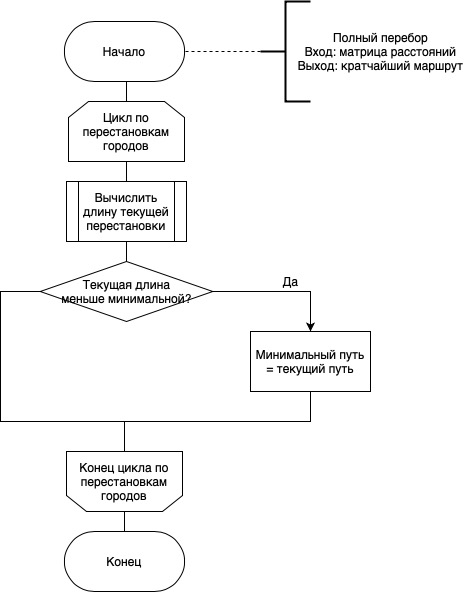
\includegraphics[scale=0.7]{dg-brute.jpg}
		\caption{Схема алгоритма полного перебора}
		\label{fig:bruteforce}
\end{figure}

\begin{figure}[H]
		\centering
		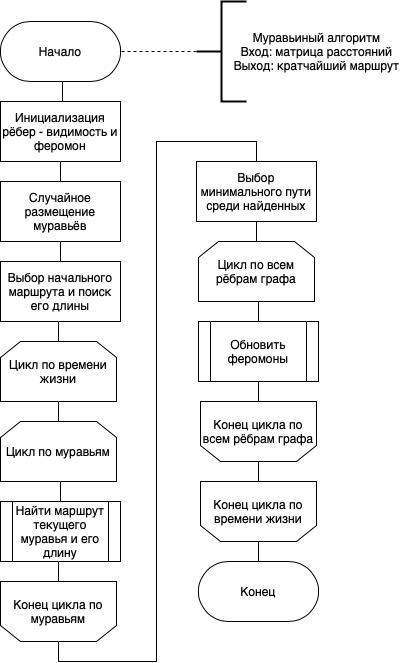
\includegraphics[scale=0.8]{dg-ant.jpg}
		\caption{Схема муравьиного алгоритма}
		\label{fig:ant}
\end{figure}

\begin{figure}[H]
		\centering
		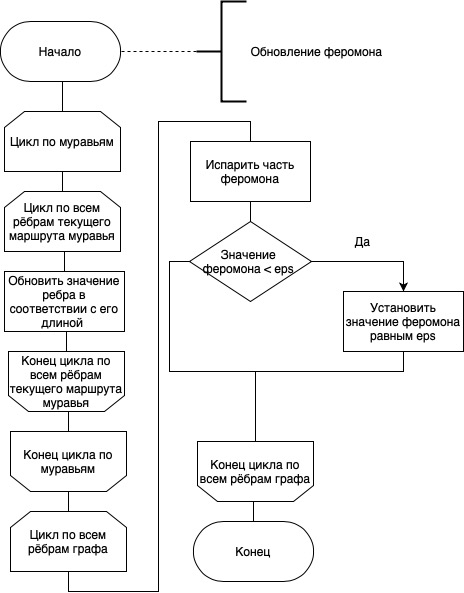
\includegraphics[scale=0.8]{dg.jpg}
		\caption{Схема алгоритма обновления феромона}
		\label{fig:ant}
\end{figure}
	
\section{Вывод из конструкторской части}
	
На основе теоретических данных, полученных аз аналитического раздела, были построенны схемы алгоритмов для решения задачи коммивояжёра.
	
\chapter{Технологическая часть}
	
В данном разделе приведены средства реализации и листинги кода.
	
\section{Средства реализации}
	В качестве языка программирования был выбран С. Данный выбор обусловлен тем, что он является языком высокого уровня. В качестве среды программирования была выбрана среда CLion. 
	
\section{Реализация алгоритмов}

В листингах 3.1 - 3.2 представлены листинги алгоритмов решения задачи коммивояжёра.

\newpage
	
\begin{lstlisting}[language=C,caption={Алгоритм полного перебора},label=code]

int nperm(size_t *seq, size_t n)
{
	size_t i = n;
	do {
		if (i < 2)
			return EXIT_FAILURE; 
		i--;
	} while (seq[i - 1] > seq[i]);
	
	size_t j;
	for (j = n; j > i && seq[i - 1] > seq[--j];) {}
		
	swp(seq + i - 1, seq + j);
	
	for (j = n; i < --j; i++)
		swp(seq + i, seq + j);
	
	return EXIT_SUCCESS;
}

int cnt_dist(mtx_t *mtx, size_t *route)
{
	int dst = 0, td;
	
	for (size_t i = 0; i < mtx->n - 1; i++)
	{
		td = mtx->data[route[i]][route[i + 1]];
		if (td < 0)
			return -1;
		
		dst += td;
	}
	
	td = mtx->data[0][mtx->n - 1];
	if (td < 0)
		return -1;
	
	dst += td;
	
	return dst;
}

int commis_voyageur_bf(mtx_t *mtx, size_t **route)
{
	*route = malloc(mtx->n * sizeof(size_t));
	size_t *tr = malloc(mtx->n * sizeof(size_t));
	
	for (size_t i = 0; i < mtx->n; i++)
		tr[i] = i;
	
	bool found = false;
	int dst, m;
	
	do {
		dst = cnt_dist(mtx, tr);
		
		if (dst >= 0 && (!found || dst < m))
		{
			found = true;
			m = dst;
			memcpy(*route, tr, mtx->n * sizeof(mtx->n));
		}
	} while (nperm(tr, mtx->n) == EXIT_SUCCESS);
	
	free(tr);
	
	if (!found)
	{
		free(*route);
		return -1;
	}
	
	return m;
}

\end{lstlisting}
	
\begin{lstlisting}[language=C,caption={Муравьиный алгоритм},label=code]

int commis_voyageur_ant(mtx_t *mtx, size_t **route, antp_t *param)
{
	mtxf_t *dist = create_mtxf(mtx->n, mtx->m);
	mtxf_t *fero = create_mtxf(mtx->n, mtx->m);
	
	ant_t *colony = malloc(mtx->n * sizeof(ant_t));
	float *p = malloc((mtx->n - 1) * sizeof(float));
	*route = malloc(mtx->n * sizeof(size_t));
	
	int L = 0;
	
	for (size_t i = 0; i < mtx->n; i++)
	{
		for (size_t j = 0; j < mtx->m; j++)
		{
			dist->data[i][j] = 1.0 / (float)mtx->data[i][j];
			
			if (mtx->data[i][j] > 0)
			{
				fero->data[i][j] = 1.0;
				L += mtx->data[i][j];
			}
			else
				fero->data[i][j] = 0.0;
		}
		
		colony[i].unvis = malloc((mtx->n - 1) * sizeof(size_t));
		colony[i].route = malloc(mtx->n * sizeof(size_t));
	}
	
	L /= 2;
	
	//start alg
	
	bool found = false;
	
	for (size_t i = 0; i < param->ANT_TIME; i++)
	{
		for (size_t ant = 0; ant < mtx->n; ant++)
		{
			colony[ant].route[0] = colony[ant].cur = ant;
			size_t c = 1;
			for (size_t j = 0; j < mtx->n; j++, c++)
			{
				if (ant == j)
					c--;
				else
					colony[ant].unvis[c - 1] = j;
			}
			
			colony[ant].unv_len = mtx->n - 1;
			size_t route_cnt = 1;
			
			while (colony[ant].unv_len)
			{
				float s = 0.0;
				for (size_t q = 0; q < colony[ant].unv_len; q++)
				{
					size_t ai = colony[ant].cur, aj = colony[ant].unvis[q];
					p[q] = powf(fero->data[ai][aj], param->ALPHA) + powf(dist->data[ai][aj], param->BETA);
					s += p[q];
				}
				float r = (float)rand() / (float)RAND_MAX;
				p[0] /= s;
				for (size_t q = 1; q < colony[ant].unv_len; q++)
				{
					p[q] /= s;
					p[q] += p[q - 1];
				}
				
				size_t q = 0;
				bool select = false;
				while (q < colony[ant].unv_len && !select)
				{
					if (r < p[q])
						select = true;
					q++;
				}

				colony[ant].route[route_cnt] = colony[ant].cur = colony[ant].unvis[q - 1];
				route_cnt++;
				
				
				size_t k;
				for (k = 0; k < colony[ant].unv_len; k++)
					if (k == q - 1)
						break;
				
				for (size_t e = k; e < colony[ant].unv_len - 1; e++)
					colony[ant].unvis[e] = colony[ant].unvis[e + 1]; 
				
				colony[ant].unv_len--;
			}
			
			int dst = cnt_dist(mtx, colony[ant].route);
			if (dst >= 0 && (!found || dst < L))
			{
				found = true;
				L = dst;
				memcpy(*route, colony[ant].route, mtx->n * sizeof(size_t));
			}
			
			colony[ant].dst = dst;
		}
		
		for (size_t i = 0; i < mtx->n; i++)
			for (size_t j = 0; j < mtx->m; j++)
				if (fero->data[i][j] > 0)
				{
					fero->data[i][j] *= 1.0 - param->RO;
					if (fero->data[i][j] < 0.1)
						fero->data[i][j] = 0.1;
				}
		
		int from, to;
		for (size_t ant = 0; ant < mtx->n; ant++)
		{
			for (size_t r = 0; r < mtx->n - 1; r++)
			{
				from = colony[ant].route[r];
				to = colony[ant].route[r + 1];
				
				fero->data[from][to] += param->Q / colony[ant].dst;
			}		

			fero->data[mtx->n - 1][0] += param->Q / colony[ant].dst;
		}
	}
	
	destroy_mtxf(dist);
	destroy_mtxf(fero);
	for (size_t i = 0; i < mtx->n; i++)
	{
		free(colony[i].unvis);
		free(colony[i].route);
	}
	free(colony);
	free(p);
	
	if (!found)
		return -1;
	
	return L;
}

\end{lstlisting}

\newpage

\section{Тестирование}

При оценивании успешности выполнения реализации алгоритмов стоит отметить, что муравьиный алгоритм не гарантирует нахождения глобального оптимума, поэтому длины полученного минимального маршрута у муравьиного алгоритма и полного перебора могут отличаться. В приведённых тестах значения длины пути у обоих алгоритмов совпали.

В таблице \ref{tab:test} приведены тестовые данные. 

\begin{table}[h!]

\caption{\label{tab:test} Тестирование реализаций алгоритмов}

	\begin{center}

		\begin{tabular}{c@{\hspace{7mm}}c@{\hspace{7mm}}c@{\hspace{7mm}}c@{\hspace{7mm}}c@{\hspace{7mm}}c@{\hspace{7mm}}}

			\hline

			Матрица смежности & Ожидаемый результат & Полученный результат\\ \hline

			\vspace{4mm}		

			$\begin{bmatrix}
			0 & 3 & 1 & 6 & 8\\
			3 & 0 & 4 & 1 & 0\\
			1 & 4 & 0 & 5 & 0\\
			6 & 1 & 5 & 6 & 1\\
			8 & 0 & 0 & 1 & 0
			\end{bmatrix}$ & 10 & 10\\

			$\begin{bmatrix}
			0 & 10 & 15 & 20\\
			10 & 0 & 35 & 25\\
			15 & 35 & 0 & 30\\
			20 & 25 & 30 & 0
			\end{bmatrix}$ & 70 & 70 \\

			
		\end{tabular}

	\end{center}


\end{table}
	
	Все тесты пройдены успешно.
	
\section{Вывод из технологической части}
	
В данном разделе были разработаны и протестированы алгоритмы решения задачи коммивояжёра.	

\chapter{Исследовательская часть}
	
В данном разделе приведен анализ характеристик разработанного ПО.
	
\section{Время выполнения алгоритмов}
	
Время выполнения алгоритма замерялось с помощью стандартной функции clock(). Для каждого размера матрицы замер проводился 10 раз, затем усреднялся. Полученные результаты приведены в таблице \ref{tab:timing}. Время указано в мс.

\begin{table}[H]

\caption{Сравнение времени исполнения алгоритмов решения задачи коммивояжера.}

	\begin{center}

		\begin{tabular}{|c|c|c|}

			\hline

			Размер графа & Полный перебор & Муравьиный алгоритм \\

			\hline
			3 & 0 & 10 \\
			4 & 0 & 20 \\
			5 & 0 & 40 \\
			6 & 0 & 30 \\
			7 & 0 & 30 \\
			8 & 20 & 50 \\
			9 & 200 & 70 \\
			10 & 2099 & 90 \\
			11 & 24272 & 110 \\
			\hline

		\end{tabular}

	\end{center}

	\label{tab:timing}

\end{table}

\section{Автоматическая параметризация}

В ходе параметризации были проанализированы следующие значения параметров алгоритма: $\alpha$ изменяется от 0 до 6, $\beta$ вычисляется как разность $6 - \alpha$; время жизни колонии от 10 до 190, коэффициент испарения от 0 до 1. Исследуется разность длины найденного пути, найденного муравьиным алгоритмом, и длины оптимального пути. 

В таблицах \ref{tab:v6} - \ref{tab:v9} приведены выборка результатов параметризации для трёх матриц расстояний размером $10\times10$. Полным перебором был посчитан оптимальный путь -- он составил 226 для первой матрицы, 249 и 166 для второй и тертьей. В столбцах разность 1 -- 3 записаны разности между результатом алгоритма и оптимальным значением пути для каждой матрицы.

\begin{table}[H]

	\caption{Выборка из результатов параметризации для матриц размером $10\times10$.}
	\label{tab:v6}
	\begin{center}

		\begin{tabular}{|c@{\hspace{7mm}}|c@{\hspace{7mm}}|c@{\hspace{7mm}}|c|c|c|}

			\hline
			$\alpha$        & Время      & $\rho$      &Разность 1    &Разность 2    &Разность 3\\
			
3.2 & 130 & 0.3 & 3 & 25 & 18 \\
3.2 & 130 & 0.6 & 0 & 25 & 15 \\
3.2 & 130 & 0.9 & 15 & 0 & 0 \\
3.2 & 190 & 0.1 & 0 & 4 & 18 \\
3.2 & 190 & 0.3 & 7 & 19 & 26 \\
3.2 & 190 & 0.6 & 26 & 27 & 18 \\
3.2 & 190 & 0.9 & 15 & 12 & 23 \\
3.6 & 10 & 0.1 & 64 & 63 & 62 \\
3.6 & 10 & 0.3 & 30 & 61 & 44 \\
3.6 & 10 & 0.6 & 32 & 32 & 19 \\
3.6 & 10 & 0.9 & 5 & 10 & 2 \\
3.6 & 70 & 0.1 & 3 & 4 & 16 \\
3.6 & 70 & 0.3 & 7 & 0 & 2 \\
3.6 & 70 & 0.6 & 10 & 0 & 13 \\
3.6 & 70 & 0.9 & 7 & 0 & 2 \\
3.6 & 130 & 0.1 & 3 & 6 & 10 \\
3.6 & 130 & 0.3 & 7 & 9 & 3 \\
3.6 & 130 & 0.6 & 0 & 4 & 8 \\
3.6 & 130 & 0.9 & 3 & 0 & 21 \\
3.6 & 190 & 0.1 & 0 & 0 & 0 \\
3.6 & 190 & 0.3 & 3 & 0 & 13 \\
3.6 & 190 & 0.6 & 0 & 0 & 16 \\
3.6 & 190 & 0.9 & 0 & 6 & 3 \\
4.0 & 10 & 0.1 & 31 & 64 & 60 \\
4.0 & 10 & 0.3 & 33 & 19 & 36 \\
4.0 & 10 & 0.6 & 7 & 21 & 18 \\
4.0 & 10 & 0.9 & 7 & 27 & 8 \\
4.0 & 70 & 0.1 & 5 & 0 & 13 \\

\hline
		\end{tabular}
	\end{center}
\end{table}

\begin{table}[H]

	\caption{Выборка из результатов параметризации для матриц размером $10\times10$.}
	\label{tab:v7}
	\begin{center}

		\begin{tabular}{|c@{\hspace{7mm}}|c@{\hspace{7mm}}|c@{\hspace{7mm}}|c|c|c|}

			\hline
			$\alpha$        & Время      & $\rho$      &Разность 1    &Разность 2    &Разность 3\\
			
4.0 & 70 & 0.3 & 3 & 0 & 10 \\
4.0 & 70 & 0.6 & 3 & 4 & 18 \\
4.0 & 70 & 0.9 & 0 & 0 & 17 \\
4.0 & 130 & 0.1 & 0 & 0 & 8 \\
4.0 & 130 & 0.3 & 0 & 0 & 25 \\
4.0 & 130 & 0.6 & 0 & 0 & 3 \\
4.0 & 130 & 0.9 & 0 & 0 & 1 \\
4.0 & 190 & 0.1 & 0 & 0 & 26 \\
4.0 & 190 & 0.3 & 0 & 0 & 8 \\
4.0 & 190 & 0.6 & 0 & 0 & 2 \\
4.0 & 190 & 0.9 & 0 & 0 & 13 \\
4.4 & 10 & 0.1 & 57 & 46 & 82 \\
4.4 & 10 & 0.3 & 34 & 4 & 13 \\
4.4 & 10 & 0.6 & 23 & 0 & 22 \\
4.4 & 10 & 0.9 & 10 & 32 & 10 \\
4.4 & 70 & 0.1 & 0 & 14 & 18 \\
4.4 & 70 & 0.3 & 7 & 0 & 21 \\
4.4 & 70 & 0.6 & 0 & 0 & 16 \\
4.4 & 70 & 0.9 & 0 & 0 & 10 \\
4.4 & 130 & 0.1 & 0 & 9 & 18 \\
4.4 & 130 & 0.3 & 0 & 0 & 16 \\
4.4 & 130 & 0.6 & 0 & 0 & 15 \\
4.4 & 130 & 0.9 & 0 & 4 & 19 \\
4.4 & 190 & 0.1 & 3 & 0 & 17 \\
4.4 & 190 & 0.3 & 0 & 0 & 18 \\
4.4 & 190 & 0.6 & 0 & 0 & 3 \\
4.4 & 190 & 0.9 & 0 & 0 & 14 \\
4.8 & 10 & 0.1 & 27 & 53 & 69 \\

			
\hline
		\end{tabular}
	\end{center}
\end{table}

\begin{table}[H]

	\caption{Выборка из результатов параметризации для матриц размером $10\times10$.}
	\label{tab:8}
	\begin{center}

		\begin{tabular}{|c@{\hspace{7mm}}|c@{\hspace{7mm}}|c@{\hspace{7mm}}|c|c|c|}

			\hline
			$\alpha$        & Время      & $\rho$      &Разность 1    &Разность 2    &Разность 3\\
			
4.8 & 10 & 0.3 & 21 & 35 & 25 \\
4.8 & 10 & 0.6 & 30 & 31 & 8 \\
4.8 & 10 & 0.9 & 0 & 0 & 23 \\
4.8 & 70 & 0.1 & 3 & 0 & 22 \\
4.8 & 70 & 0.3 & 0 & 0 & 20 \\
4.8 & 70 & 0.6 & 3 & 6 & 2 \\
4.8 & 70 & 0.9 & 3 & 10 & 3 \\
4.8 & 130 & 0.1 & 7 & 4 & 15 \\
4.8 & 130 & 0.3 & 0 & 4 & 13 \\
4.8 & 130 & 0.6 & 0 & 6 & 19 \\
4.8 & 130 & 0.9 & 0 & 9 & 3 \\
4.8 & 190 & 0.1 & 4 & 0 & 18 \\
4.8 & 190 & 0.3 & 0 & 4 & 10 \\
4.8 & 190 & 0.6 & 0 & 0 & 5 \\
4.8 & 190 & 0.9 & 0 & 0 & 15 \\
5.2 & 10 & 0.1 & 44 & 19 & 60 \\
5.2 & 10 & 0.3 & 35 & 27 & 3 \\
5.2 & 10 & 0.6 & 49 & 49 & 39 \\
5.2 & 10 & 0.9 & 5 & 35 & 38 \\
5.2 & 70 & 0.1 & 15 & 19 & 13 \\
5.2 & 70 & 0.3 & 10 & 14 & 16 \\
5.2 & 70 & 0.6 & 12 & 10 & 21 \\
5.2 & 70 & 0.9 & 12 & 28 & 0 \\
5.2 & 130 & 0.1 & 0 & 9 & 16 \\
5.2 & 130 & 0.3 & 0 & 27 & 6 \\
5.2 & 130 & 0.6 & 7 & 6 & 15 \\
5.2 & 130 & 0.9 & 10 & 20 & 2 \\
5.2 & 190 & 0.1 & 0 & 9 & 17 \\

\hline
		\end{tabular}
	\end{center}
\end{table}

\begin{table}[H]

	\caption{Выборка из результатов параметризации для матриц размером $10\times10$.}
	\label{tab:v9}
	\begin{center}

		\begin{tabular}{|c@{\hspace{7mm}}|c@{\hspace{7mm}}|c@{\hspace{7mm}}|c|c|c|}

			\hline
			$\alpha$        & Время      & $\rho$      &Разность 1    &Разность 2    &Разность 3\\
5.2 & 190 & 0.3 & 0 & 4 & 15 \\
5.2 & 190 & 0.6 & 7 & 23 & 2 \\
5.2 & 190 & 0.9 & 4 & 13 & 0 \\
5.6 & 10 & 0.1 & 52 & 69 & 62 \\
5.6 & 10 & 0.3 & 58 & 63 & 86 \\
5.6 & 10 & 0.6 & 66 & 60 & 46 \\
5.6 & 10 & 0.9 & 88 & 57 & 22 \\
5.6 & 70 & 0.1 & 19 & 47 & 21 \\
5.6 & 70 & 0.3 & 27 & 56 & 31 \\
5.6 & 70 & 0.6 & 31 & 36 & 25 \\
5.6 & 70 & 0.9 & 23 & 42 & 49 \\

\hline
		\end{tabular}
	\end{center}
\end{table}


\section{Вывод из исследовательской части}

При небольших размерах графа (от 3 до 8) алгоритм полного перебора выигрывает по времени у муравьиного. Однако, при увеличении размера графа (от 9 и выше), ситуация меняется в обратную сторону: муравьиный алгоритм начинает значительно выигрывать по времени у алгоритма полного перебора. На размерах графа 11, муравьиный алгоритм работает в 220 раз быстрее.

При параметризации в качестве тестовых данных использовались матрицы расстояний с одинаковым разбросом длин рёбер. Наиболее стабильные результаты автоматической параметризации получаются при наборе $\alpha = 3.6..4.8$, $\beta = 6 - \alpha$, $\rho = 0.6$. При времени жизни колонии, превышающем число городов, результат является более точным.

Тогда можно сделать вывод, что при числе городов, меньшем девяти стоит использовать алгоритм полного перебора для получения точного результата. Для иного числа городов стоит использовать муравьиный алгоритм с выявленными параметрами. Однако нужно понимать, что результат работы муравьиного алгоритма не всегда является оптимальным маршрутом.

\chapter*{Заключение}
\addcontentsline{toc}{chapter}{Заключение}
	
В рамках данной лабораторной работы лабораторной работы была достигнута её цель: изучен муравьиный алгоритм и приобретены навыки параметризации методов на примере муравьиного алгоритма. Также выполнены следующие задачи:
	
\begin{itemize}
	\item решена задача коммивояжера при помощи алгоритма полного перебора и муравьиного алгоритма;
	\item реализованы алгоритмы полного перебора и муравьиный алгоритм для решения задачи коммивояжёра;
	\item замерено и сравнено время выполнения реализаций алгоритмов;
	\item проведена параметризация реализации муравьиного алгоритма;
	\item сделаны выводы на основе проделанной работы.
\end{itemize} 

\addcontentsline{toc}{chapter}{Литература}
\bibliographystyle{utf8gost705u}  % стилевой файл для оформления по ГОСТу
\bibliography{51-biblio}          % имя библиографической базы (bib-файла)
	
\end{document}